\documentclass[a4paper,10pt]{scrartcl}
\usepackage[utf8]{inputenc}
\usepackage[T1]{fontenc}
\usepackage{lmodern}
\usepackage[german]{babel}
\usepackage{listings}
\usepackage{color}
\usepackage[parfill]{parskip}
\usepackage{graphicx}
\lstset{basicstyle=\ttfamily}
\renewcommand{\lstlistingname}{Eintrag}

\begin{document}
\title{Entwicklung einer Hard- und Softwarebasis zur Automatisierung des Traxxas Summit}
\author{Pascal Ernst\\
  70302367 \\
  Ostfalia Hochschule für angewandte Wissenschaften \\
  Projektrealisierung mit Hilfe von: \\
  Edgar Wendler, Dennis Gieger}
\date{November 2015}
\maketitle

\newpage

\section{Komponenten}

  \subsection{Traxxas Summit}

    \begin{figure}[ht!]
      \centering
      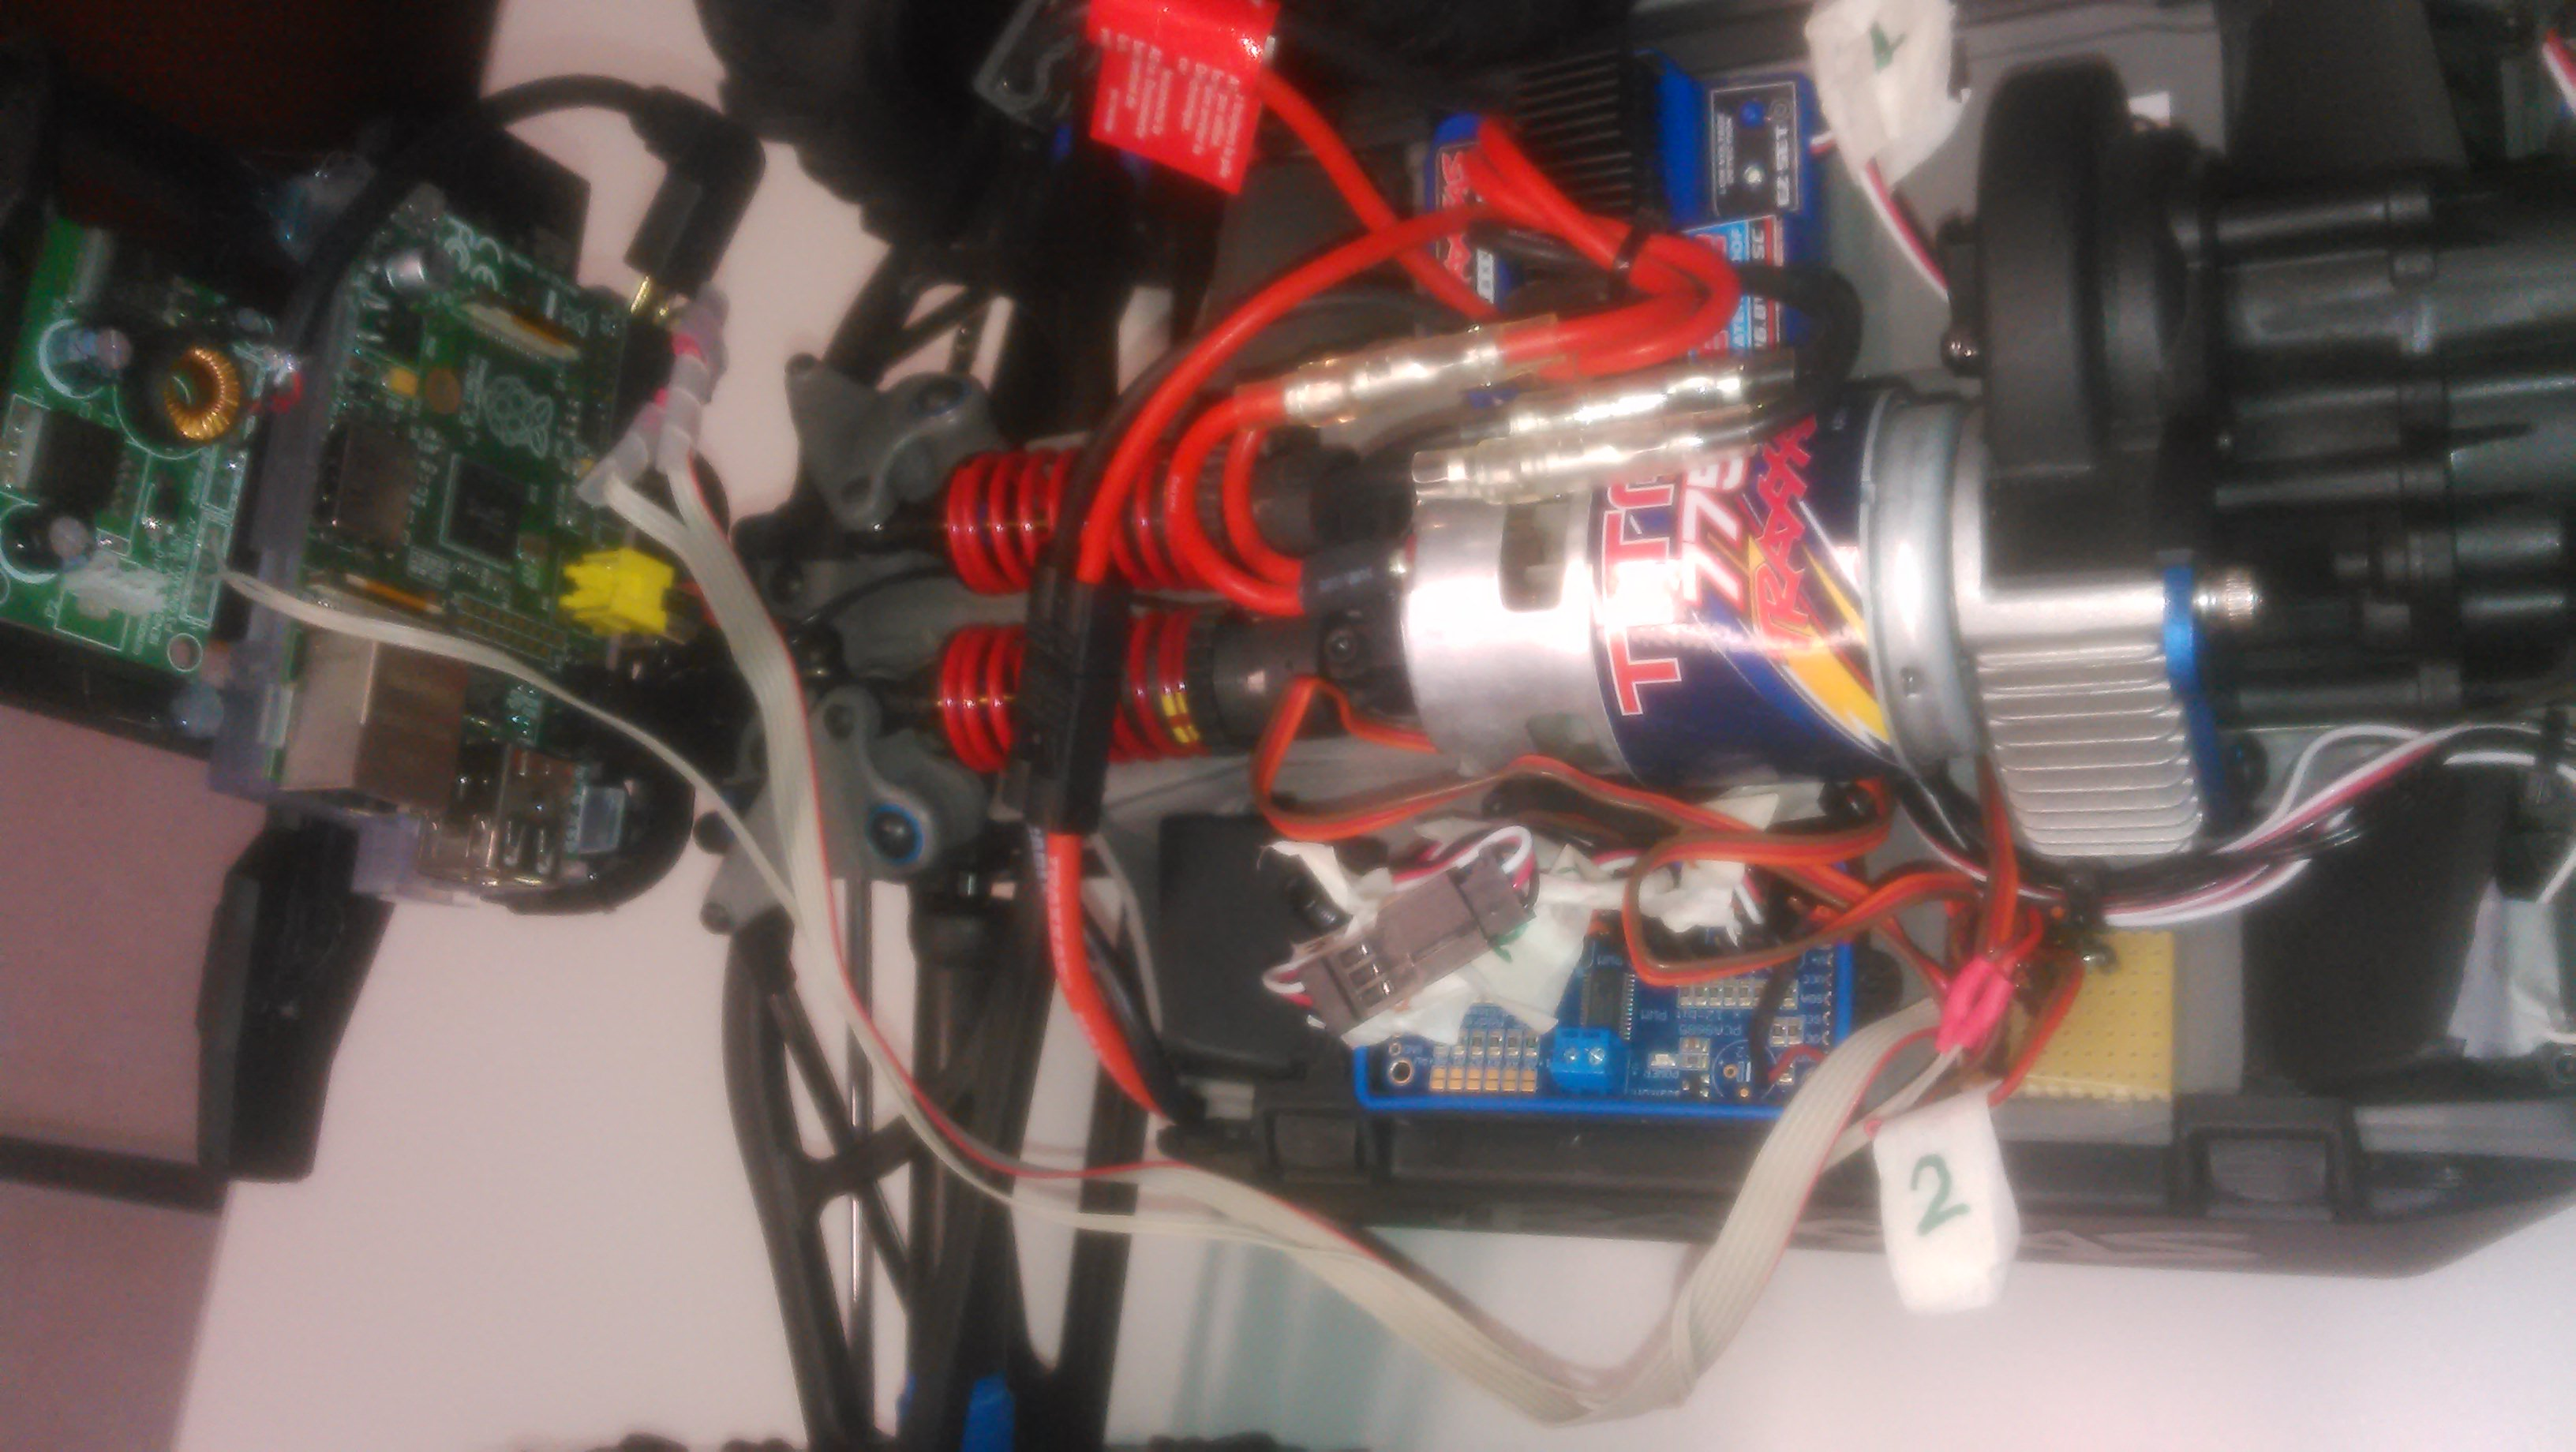
\includegraphics[width=100mm]{pics/hardware.jpg}
      \caption{Der Traxxas Summit mit den eingebauten Komponenten}
    \end{figure}

    Der Traxxas Summit ist ein per Funk gesteuertes Modell-Auto vom Hersteller
    Traxxas.
    Es besitzt unter anderem Servos zum Ansteuern der Funktionen und einen mit
    PWM gesteuerten ESC mit eingebautem BEC (leitet Strom des ESCs weiter an die
    Servos).

    Um diesen zu automatisieren, wird das Empfänger-Modul, das die Funkbefehle
    zur Steuerung des Autos empfängt, entfernt.
    Die Anschlüsse, die von dem Modul zum ESC sowie zu den Servos führten,
    können direkt für den Adafruit Servo Driver benutzt werden.

    Einige Servos können übersteuert werden weil daran angeschlossene
    Komponenten nur einen Teil des Bewegungsraumes benutzen und blockieren /
    stoppen wenn der Servo sich darüber hinaus bewegt.
    Hier muss für die einzelnen Servos software-seitig der Spielraum der
    PWM-Signale ausgetestet werden, was im Sturo-Programm für den Traxxas Summit
    bereits geschehen ist.

    \newpage

  \subsection{Raspberry Pi}

    \begin{figure}[ht!]
      \centering
      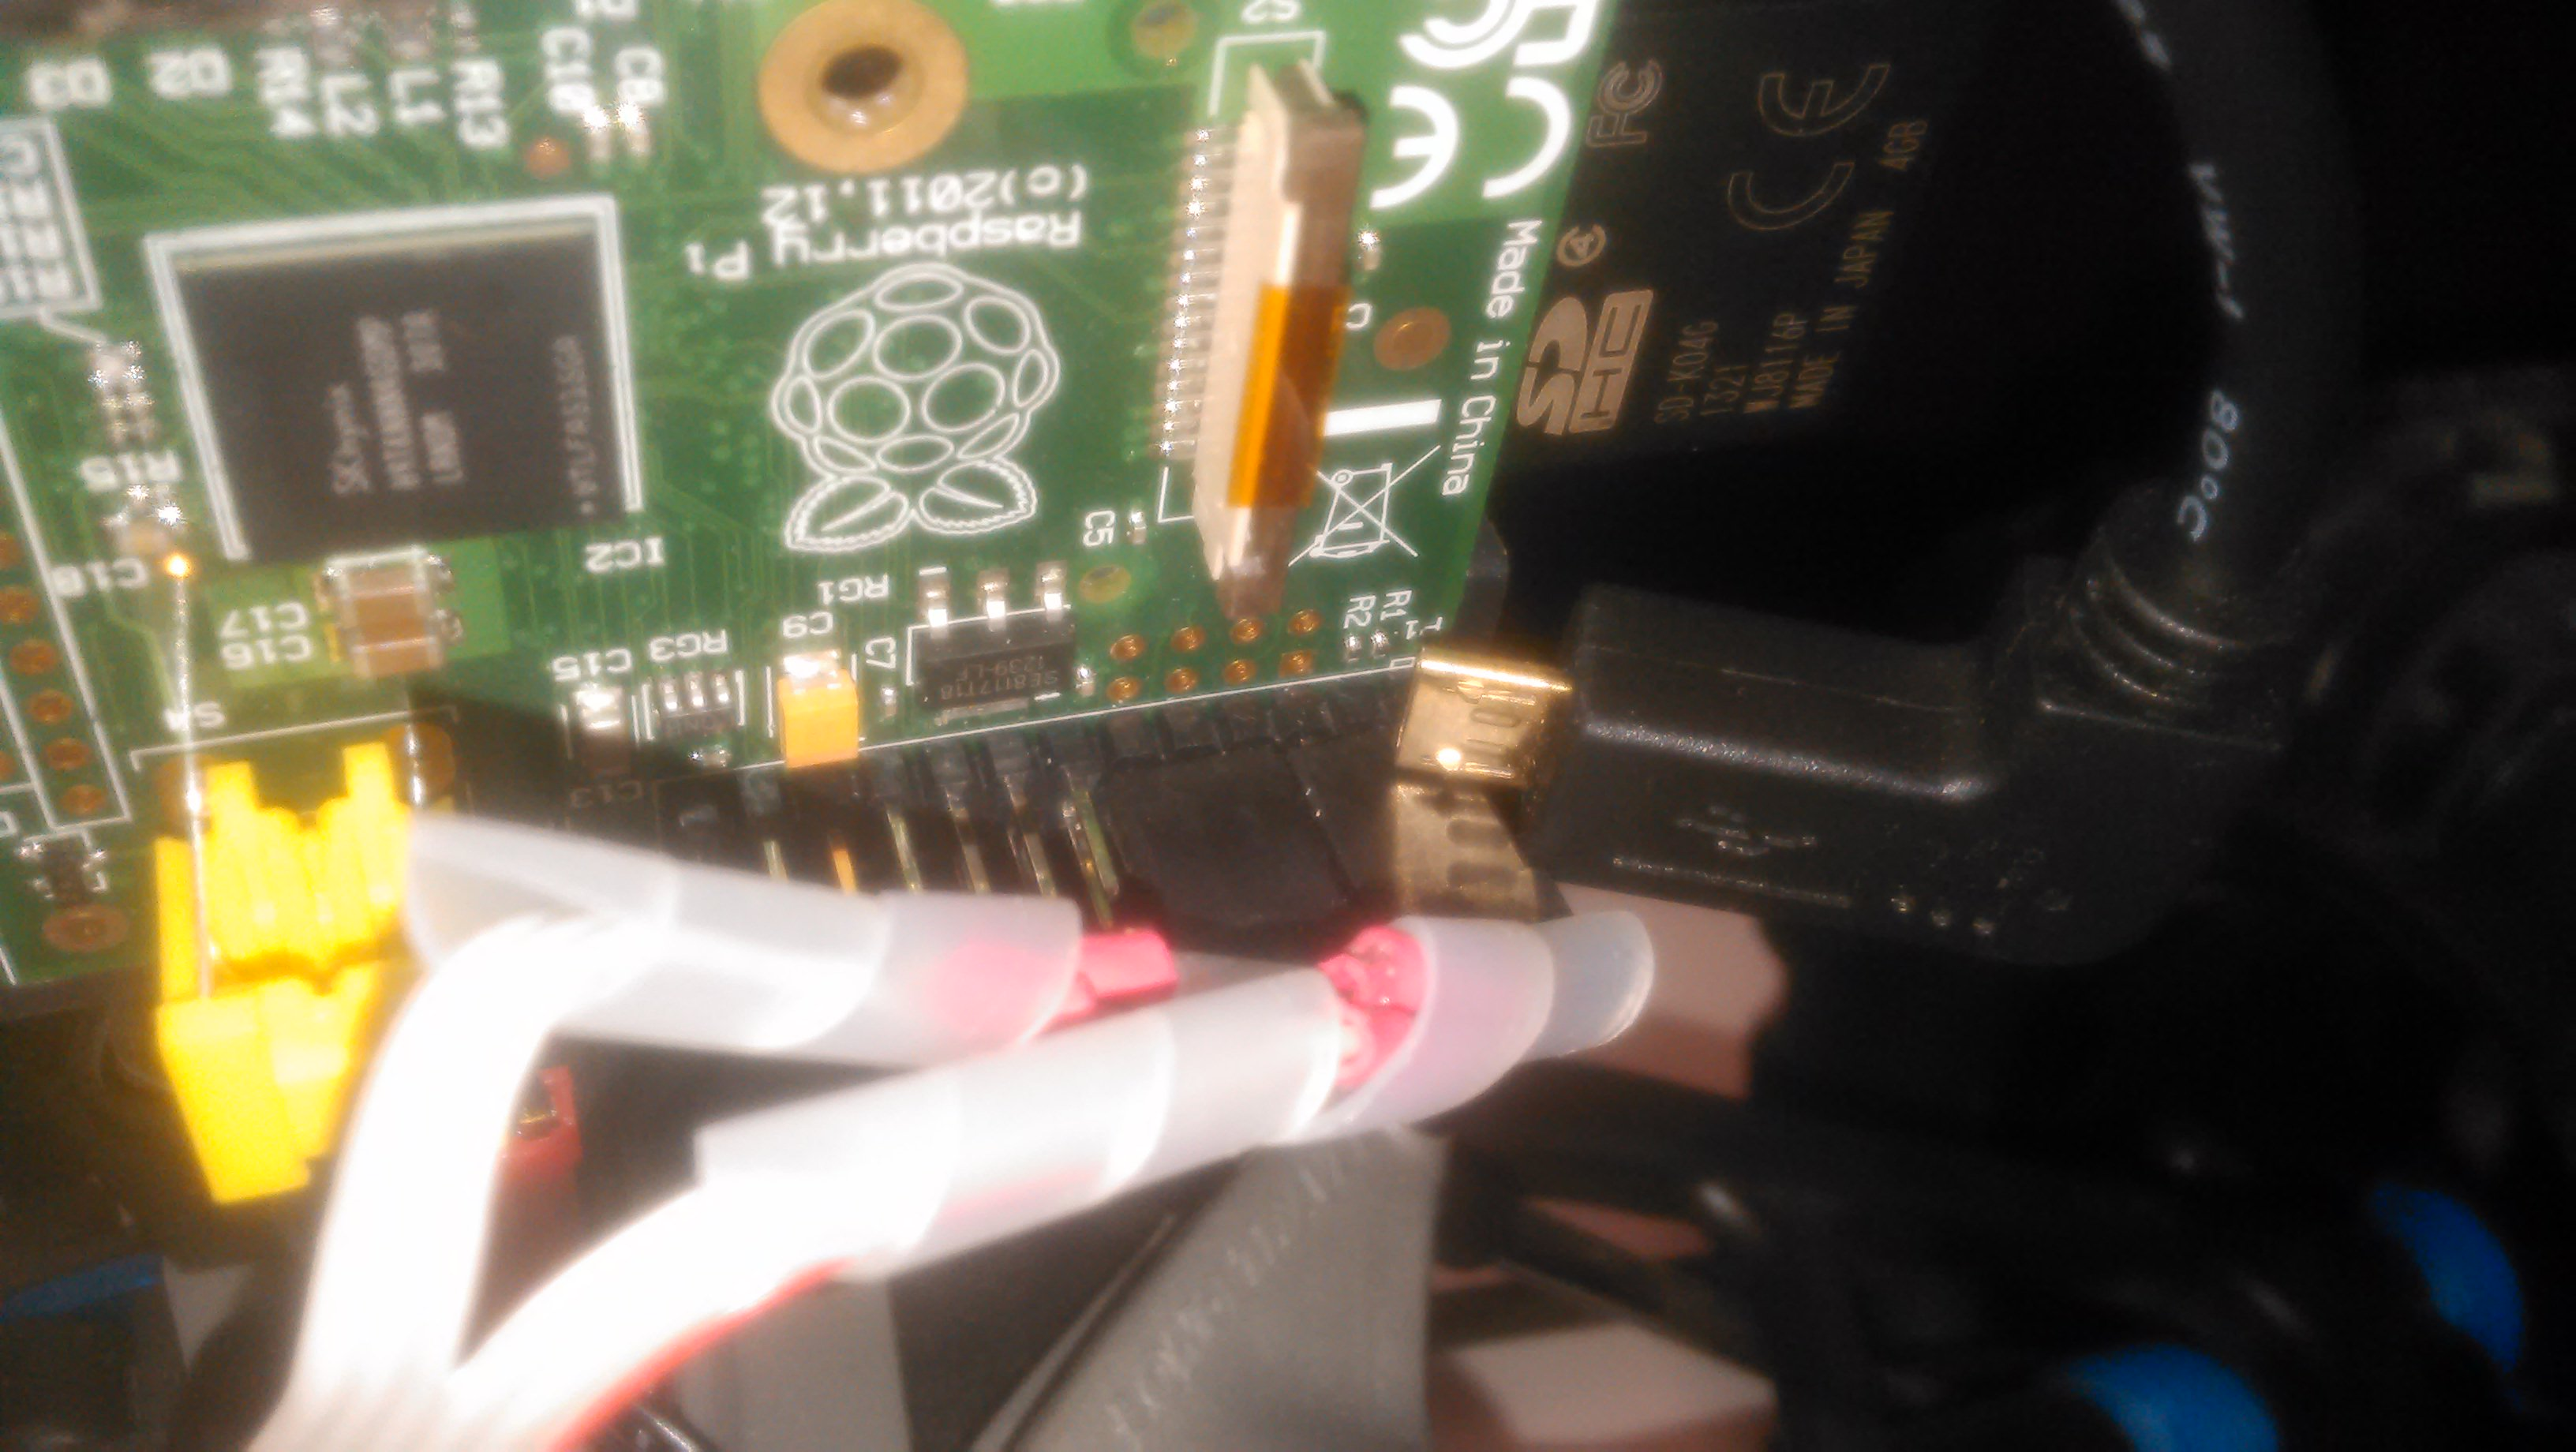
\includegraphics[width=100mm]{pics/rpi.jpg}
      \caption{Der Raspberry Pi mit den GPIO-Anschlüssen des Servo Drivers}
    \end{figure}

    Der Raspberry Pi ist ein günstiger Mini-Computer.
    Er ist mit dem Adafruit Servo Driver verbunden und führt das Programm Sturo
    aus, das eine Automatisierung der Fahrt des Autos ermöglicht.
    Es können noch weitere Komponenten, wie zum Beispiel ein Ultraschall-Sensor,
    mit dem Raspberry Pi verbunden werden.

  \subsection{Adafruit 16-Channel 12-Bit Servo Driver}

    \begin{figure}[ht!]
      \centering
      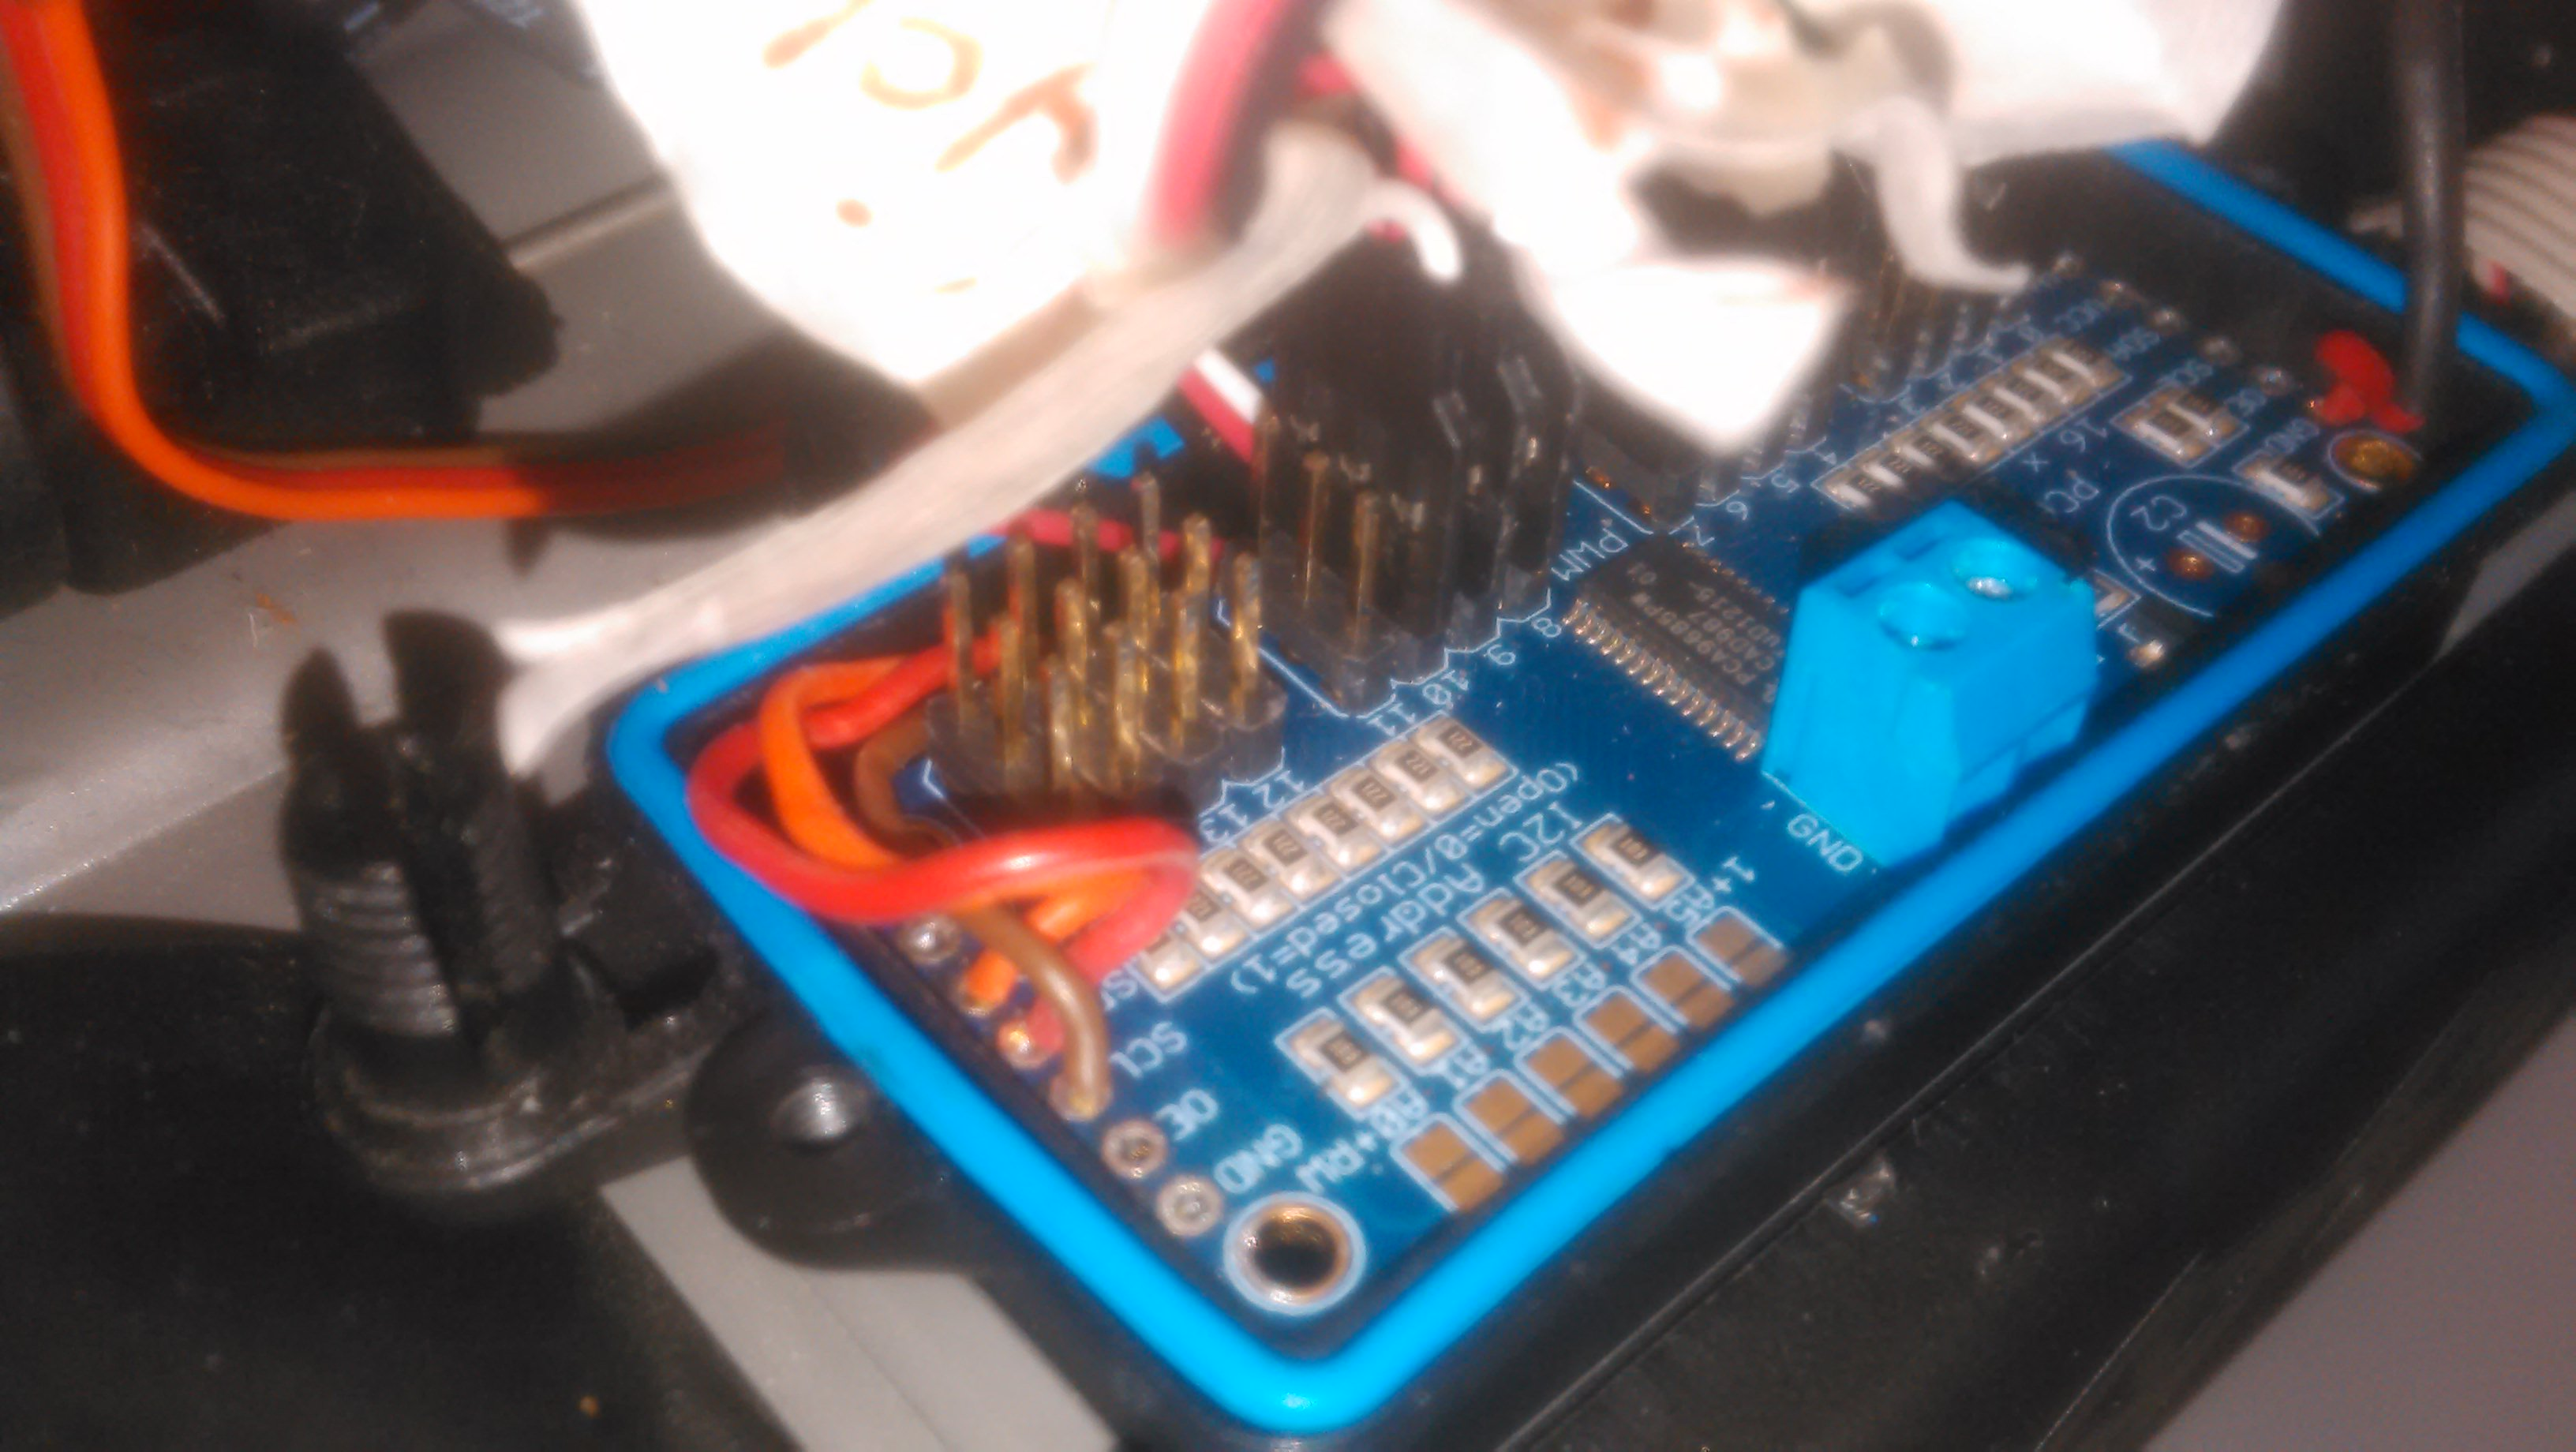
\includegraphics[width=100mm]{pics/servo_driver.jpg}
      \caption{Der Servo Driver, eingelassen in die Box für den Empfänger}
    \end{figure}

    Dieser Servo Driver \cite{adafruitmod} erlaubt die Kontrolle der einzelnen
    Servos und des ESCs mithilfe von PWM.
    Er wird über I2C an den Raspberry Pi angeschlossen und erhält von diesem die
    Ansteuerungs-Befehle.

    Er besitzt 16 Anschlüsse (Ports) für jeweils einen Servo.
    Diese sind von 0 bis 15 durchnummeriert und können in der Software
    angesprochen werden.
    Für Sturo sind die folgenden Anschlüsse belegt:

    \begin{lstlisting}
Port 0    Lenkung Servo 1
Port 1    Lenkung Servo 2
Port 4    ESC (Geschwindigkeit)
Port 8    Gangschaltung
Port 9    Vordere Differentialsperre
Port 10   Hintere Differentialsperre
    \end{lstlisting}

    Weitere Anschlüsse, wie z.B. die Stromversorgung für den Spannungswandler,
    können beliebig auf die verbleibenden Ports verteilt werden.

  \subsection{Spannungswandler}

    \begin{figure}[ht!]
      \centering
      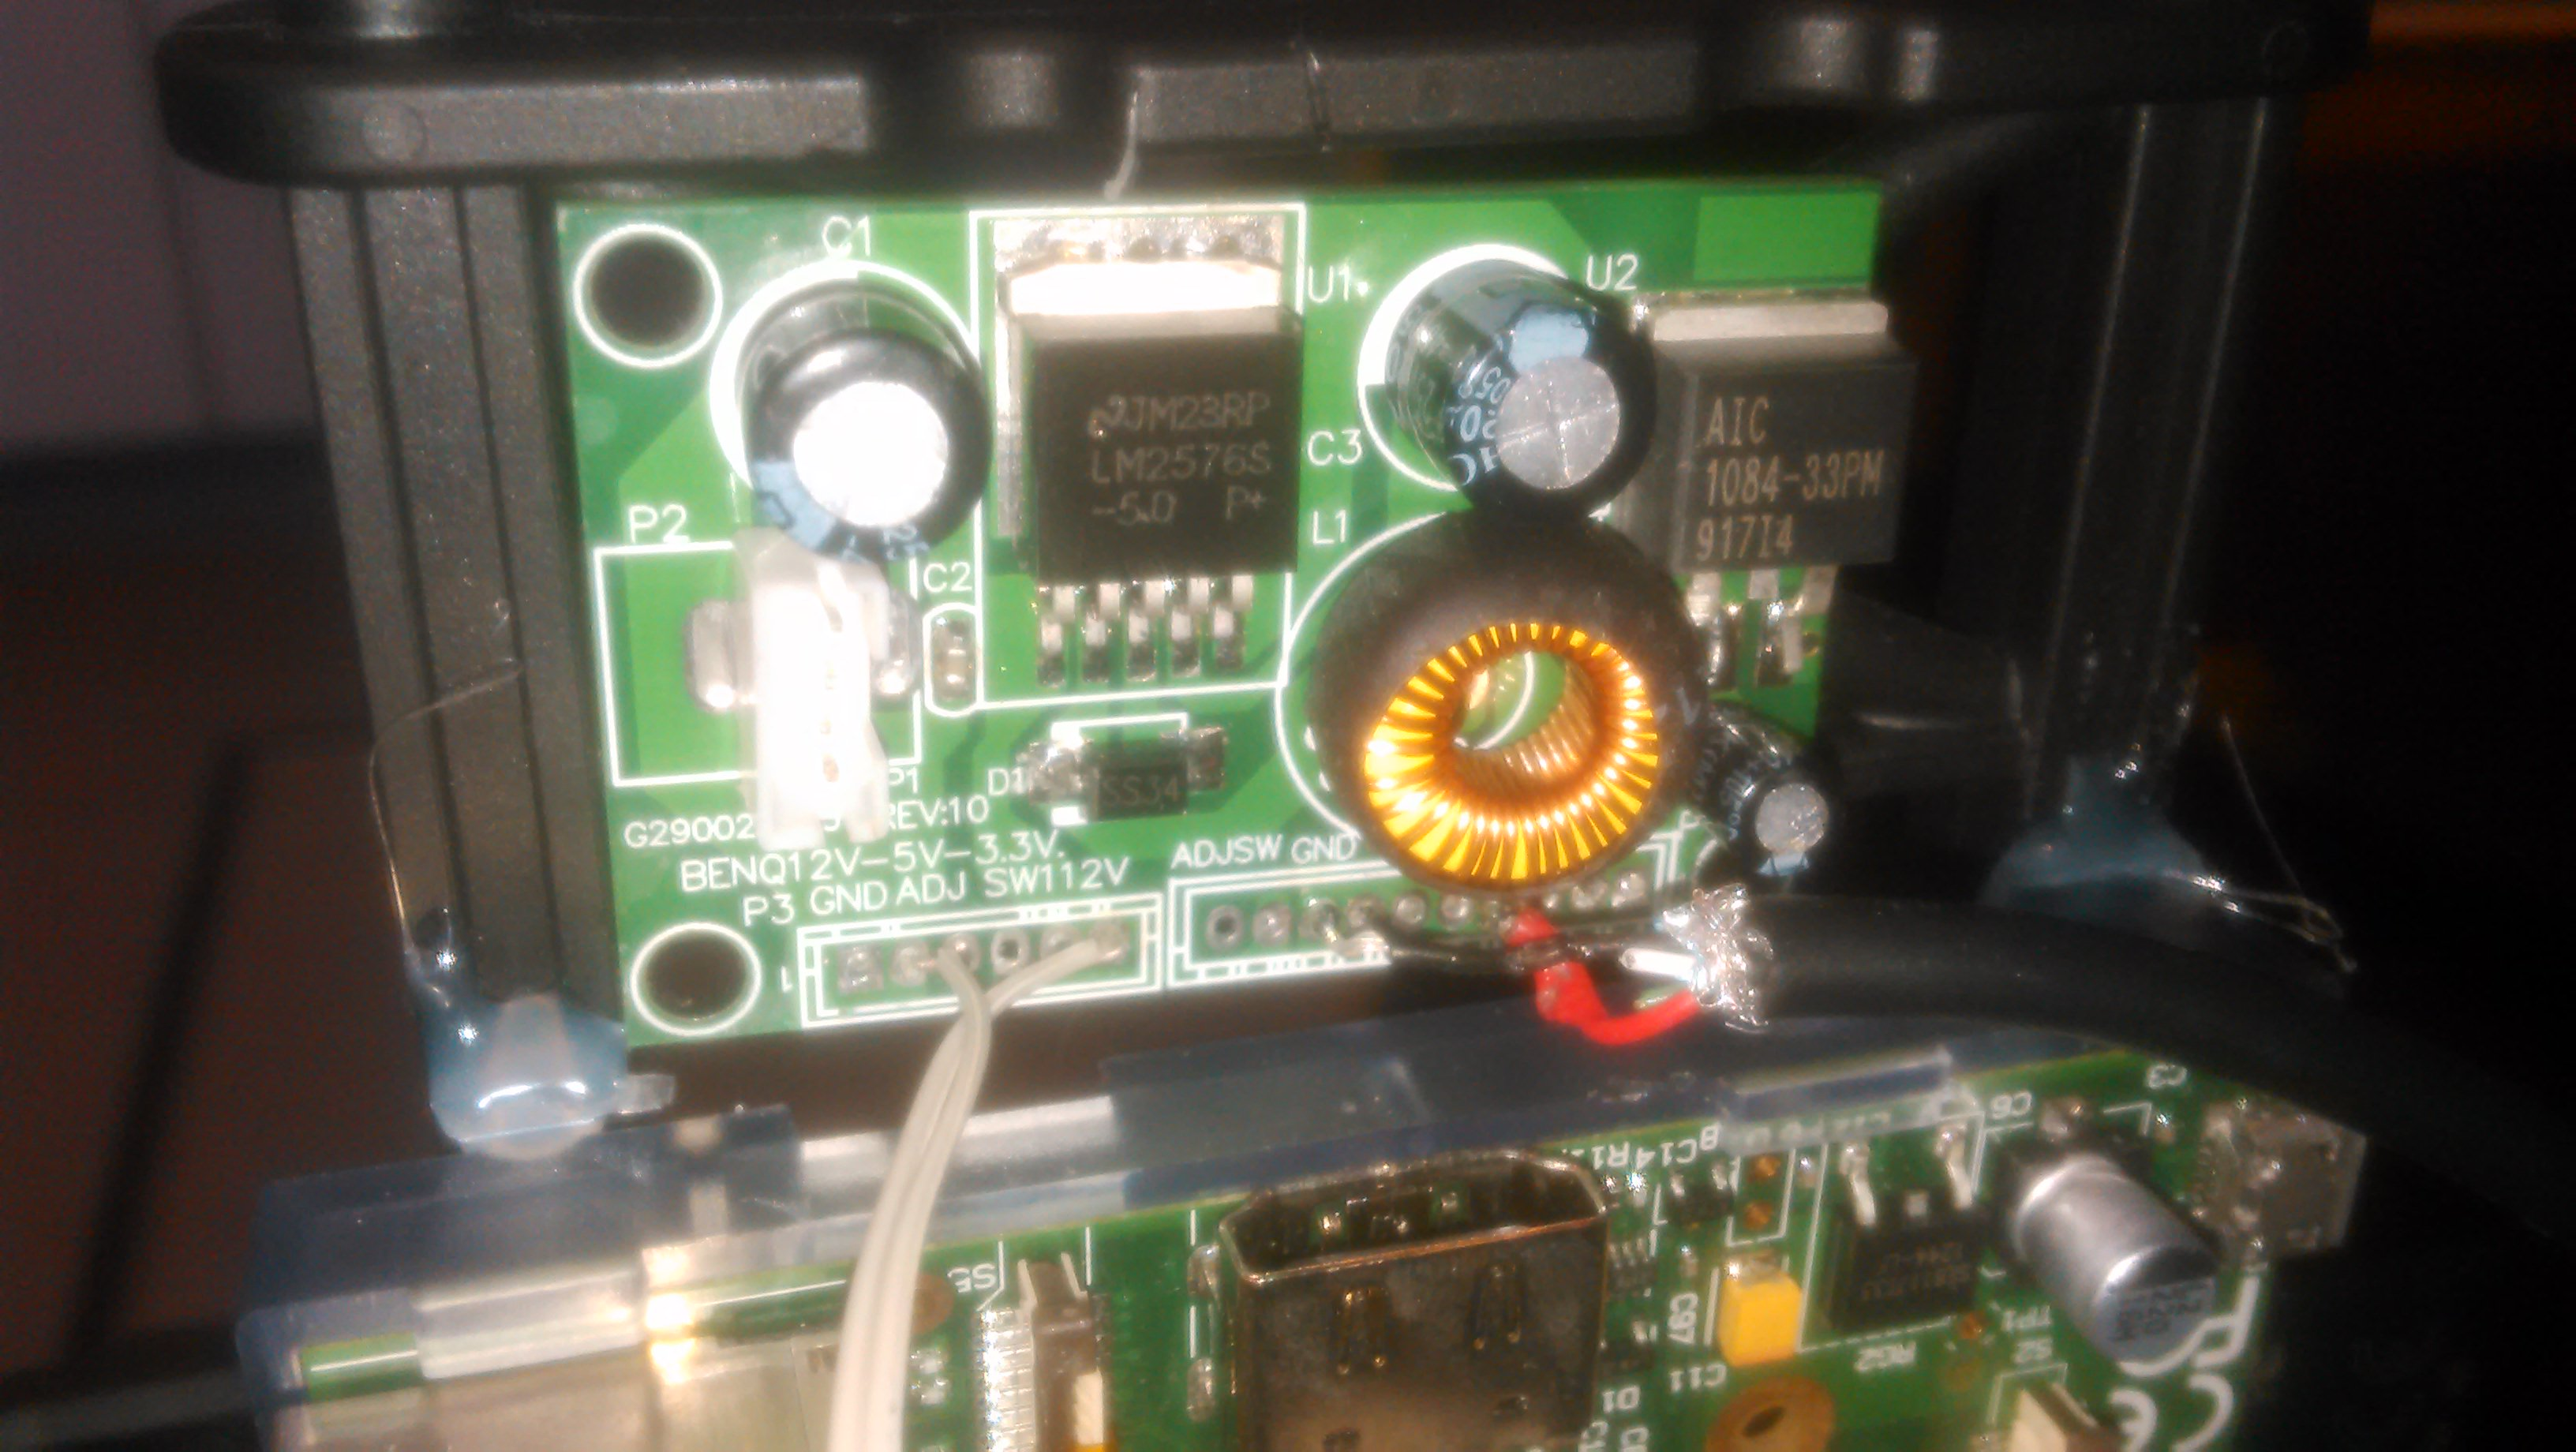
\includegraphics[width=100mm]{pics/spannungswandler.jpg}
      \caption{Der Spannungswandler mit Micro-USB Anschluss links abgehend}
    \end{figure}

    Der Spannungswandler wandelt die Spannung (ungefähr 6V), die der BEC aus den
    Akkus des Autos den Servos zur Verfügung stellt, in eine für den
    Raspberry Pi nutzbare Spannung (5V) um.

    Im Projekt haben wir den BenQ DC 12V to 5V/3.3V Converter benutzt.
    Der 12V-Eingang wird an einen \lstinline{V+}-Anschluss am Servo Driver
    angeschlossen.
    Um Spannungsschwankungen durch die unterschiedliche Servo-Belastung zu
    minimieren, wird hier noch ein Kondensator dazwischen eingefügt.
    Der \lstinline{GND} Eingang wird ebenfalls an einen
    \lstinline{GND}-Anschluss (für die Servos, nicht dem Raspberry Pi) des Servo
    Drivers angeschlossen.

    Um den Spannungswandler an den Raspberry Pi anzuschließen, wurde ein
    Mikro-USB Kabel an einer Seite aufgeschnitten um das rote Kabel an den 5V
    Ausgang und das schwarze Kabel an den \lstinline{GND} Ausgang des
    Spannungswandlers anzuschließen.

    Nun wird der Raspberry Pi über den normalen Mikro-USB Anschluss mit Strom
    versorgt.

  \subsection{Ultraschallsensor}

    Der Ultraschallsensor erlaubt dem Programm die Entdeckung von Hindernissen
    und die korrekte Reaktion darauf.
    Das Projekt benutzt den Ultraschallsensor mit der Nummer
    \lstinline{HC-SR04}.

    Der Sensor hat vier Anschlüsse;
    \lstinline{GND} und \lstinline{VCC} können direkt an den Raspberry Pi
    angeschlossen werden.
    \lstinline{Echo} und \lstinline{Trig} können an beliebige GPIO Anschlüsse
    angebracht werden, Sturo geht jedoch davon aus das sie jeweils auf
    \lstinline{GPIO 27} und \lstinline{GPIO 22} angeschlossen sind.

    Sollte VCC an den 5V Anschluss des Raspberry Pis angeschlossen sein
    (Die 3,3V werden für I2C benutzt), muss man noch einen 1K Widerstand
    zwischen \lstinline{Echo} und den Raspberry Pi anbringen.

\section{Aufsetzen des Raspberry Pis}

  Das Betriebssystem des Raspberry Pis benötigt etwas Zusatzsoftware, um über
  das I2C-Interface mit dem Adafruit 16 Channel Servo Driver kommunizieren zu
  können.
  Im folgenden wird von Raspbian als Betriebssystem ausgegangen.
  Dieses kann von \lstinline{https://www.raspberrypi.org/} kostenlos
  heruntergeladen und dann auf die SD-Karte für den Raspberry Pi überspielt
  werden.

  \paragraph{I2C Software} Zuerst wird die Software zum Ansteuern des PWM-Moduls
  installiert:
    \begin{lstlisting}[language=sh]
sudo apt-get update
sudo apt-get install python-smbus
sudo apt-get install i2c-tools
    \end{lstlisting}

    Dann muss \lstinline{/etc/modprobe.d/raspi-blacklist.conf} überprüft werden.
    Falls die Datei die Zeile \lstinline{blacklist i2c-bcm2708} enthält, mit
    \lstinline{#} auskommentieren.
    Nun noch in \lstinline{/etc/modules} die Zeilen
    \begin{lstlisting}
i2c-dev
i2c-bcm2708
    \end{lstlisting}

    hinzufügen und den Raspberry Pi neustarten.

    Jetzt wird der Adafruit 16 Channel Servo Driver an die GPIO-Pins des
    Raspberry Pis angeschlossen.
    Mithilfe von \lstinline{sudo i2cdetect -y 0} bzw.
    \lstinline{sudo i2cdetect -y 1} (je nach Baureihe des Raspberry Pis) kann
    die Verbindung zwischen dem Servo Driver und dem Raspberry Pi überprüft
    werden.\cite{adafruitlearn}

  \paragraph{Sturo} Nun richten wir das Programm zur Steuerung des RC-Autos ein.

    Die aktuelle Version des Programmes befindet sich momentan auf Github:

    \begin{lstlisting}
wget https://github.com/linucc/sturo
cd sturo
chmod +x sturo_start.sh
    \end{lstlisting}

    Das Programm Sturo benötigt Python 2.7 und muss für Funktionen wie Sensoren
    privilegiert ausgeführt werden.
    Nun soll der Raspberry Pi Sturo direkt nach dem Bootvorgang ausführen.

    Dazu editiert man die Datei \lstinline{/etc/inittab}, sodass der Login beim
    Booten automatisch ausgeführt wird:

    Die Zeile \lstinline{1:2345:respawn:/sbin/getty 115200 tty1} wird mit
    \lstinline{#} auskommentiert.
    Dann kann man direkt darunter in einer neuen Zeile diesen Code einfügen:
    \begin{lstlisting}
1:2345:respawn:/bin/login -f pi tty1 </dev/tty1 >/dev/tty1 2>&1
    \end{lstlisting}
    Beim Login ist man nun als Benutzer \lstinline{Pi} eingeloggt.
    \cite{opentech}

    Jetzt wird die Skriptdatei aufgerufen, indem am Ende der Datei
    \lstinline{/etc/profile} die Zeile
    \begin{lstlisting}
. /home/pi/sturo/sturo_start.sh
    \end{lstlisting}
    eingefügt wird.

    Damit Sturo erweiterte Funktionen benutzen kann, muss es privilegiert
    mithilfe von \lstinline{sudo} ausgeführt werden.
    Hier wird momentan je nach Betriebssystem noch nach einem Passwort gefragt,
    sodass sich das Programm nicht automatisch startet.

    Um dies zu umgehen, können wir das \lstinline{setuid bit} auf den Nutzer
    \lstinline{root} setzen oder die \lstinline{/etc/sudoers} Datei mithilfe von
    \lstinline{visudo} editieren und folgende Zeile an das Ende fügen:
    \begin{lstlisting}
pi ALL=NOPASSWD: /usr/bin/python
    \end{lstlisting}

    Nun wird beim Ausführen von Python mit \lstinline{sudo} nicht mehr nach dem
    Passwort gefragt.

    Das führt in Kombination mit dem Auto-Login zu einem sehr unsicheren System,
    was für dieses Projekt aber erstmal unwichtig ist.

\section{Sturo Software Implementierung}

  \subsection{Externer Sourcecode}
    Sturo benutzt die Module \lstinline{adafruit_servo_driver} und
    \lstinline{adafruit_i2c} für Python, welche eine grundlegende Ansteuerung
    des Servo Drivers ermöglichen. \cite{adafruitlearn}

    Weiterhin wurde das Modul \lstinline{usonic} eingebunden, um die Messdaten
    aus dem Ultraschallsensor abzulesen. \cite{ultrasonic}

    Der Code dieser Module ist unter \lstinline{lib} zu finden.

  \subsection{ServoControl}

    Das \lstinline{ServoControl} Modul abstrahiert die Arbeit mit der PWM.

    Es enthält zum einen die Klasse \lstinline{SummitPWM}, die die Attribute des
    Adafruit Servo Drivers festlegt und anhand eines übergebenen
    \lstinline{Servo} die Pulslänge zur Ansteuerung des Servos ändern kann,
    indem es mit diesem Servo Drivers kommuniziert.

    Zum anderen ist dort die Klasse \lstinline{Servo} zu finden, die einen
    spezifischen Servo repräsentiert.
    Dort wird festgelegt, wie dieser Servo angesprochen wird:
    \begin{lstlisting}
class Servo(object):
  """Represents a pwm-controlled servo"""

  def __init__(self):
    self.range_min = 219   # 1ms wide pulse
    self.range_max = 438   # 2ms wide pulse
    self.pwm_port = 0   # The port the servo can be accessed from

  [...]
    \end{lstlisting}

    Für jeden Servo wird eine eigene Klasse definiert, die von \lstinline{Servo}
    erbt und dessen Attribute anpasst.
    So wird für die vordere Differentialsperre die Klasse \lstinline{FrontLocker}
    definiert.
    Hier wird der Port gesetzt der den Adafruit Servo Driver mit diesem Servo
    verbindet.
    Außerdem wird die maximale und minimale Pulslänge eingeschränkt, weil die
    Mechanik der vorderen Differentialsperre nicht auf die volle Bewegung des
    Servos ausgelegt ist.
    \begin{lstlisting}
[...]
class FrontLocker(Servo):
    """The front locker servo of the Summit"""
    def __init__(self):
        super(FrontLocker, self).__init__()
        self.pwm_port = 9
        # This servos movement is quite restricted
        self.pwm_range_adjust(0.7, 0.9)
[...]
    \end{lstlisting}

  \subsection{CarAttributes}

    Die Klasse \lstinline{CarAttributes} abstrahiert die Kontrolle der Traxxas
    Summit Servos weiter indem die Kontrolle der einzelnen Servos in
    allgemeinere Methoden gepackt werden und die Parameter sinnvoll angepasst
    werden.

    So gibt es eine Methode, die die Lenkung des Autos steuert.
    Da die Reifenauslenkung von zwei Servos gleichzeitig gesteuert werden
    (eines für jedes der frontalen Räder) steuert diese Methode gleich zwei der
    Servos an.
    Statt eines Parameters mit dem Wert zwischen 0 (minimale Pulslänge) und 1
    (maximale Pulslänge) zu erwarten, erwartet diese Funktion einen Winkel:
    Eine Float zwischen -45 und 45:
    \begin{lstlisting}
[...]
    def set_steering(self, angle):
        """Changes the angle of the wheels

        Arguments:
        angle -- between -45 and 45
        """
        val = (float(angle) + 45) / 90
        self.pwm.servo_set(self.servo_steering1, val)
        self.pwm.servo_set(self.servo_steering2, val)
[...]
    \end{lstlisting}

  \subsection{Driver}

    In den bisher genannten Code-Segmenten wurde die Operation des Autos
    abstrahiert.
    Die Klasse \lstinline{Driver} soll dagegen beweisen, dass mithilfe der
    bisher eingeführten Methoden eine einfache Automatisierung des Autos
    möglich ist.
    Es benutzt die Klasse \lstinline{CarAttributes}, um die Mechanik des Autos
    zu kontrollieren.

    Die Methode \lstinline{evaluate} liest einen Wert aus dem Ultraschallsensor
    aus.
    Basierend darauf wird ein \lstinline{Mode} gesetzt, der die nächste Aktion
    des Autos angibt, zum Beispiel \lstinline{Mode.REVERSE}.

    Die Methode \lstinline{drive} ruft dann, anhand des Moduses der in
    \lstinline{evaluate} generiert wird, die entsprechenden Operationen auf
    damit der Traxxas Summit angemessen auf die von den Servos erhaltenen
    Informationen reagiert.

\section{Herausforderungen}

  \subsection{Betrieb des Motors}

    Anfangs war es nicht möglich, den ESC so anzusteuern, dass dieser wiederum
    den Motor aktiviert.
    Der Grund dafür ist ein Sicherheitsfeature welches direkt in den ESC
    eingebaut wurde.
    Es erwartet nach dem Einschalten ein PWM-Signal mit einer Pulslänge von
    50\% der gesamten Pulslängenreichweite (1.5ms) und schaltet dann erst in
    einen Modus, mit dem die Geschwindigkeit des Fahrzeuges gesetzt werden kann.

    Dies haben die Spezifikationen von Traxxas über den Traxxas Summit nicht
    angegeben.
    Sie haben jedoch die Taktung des PWM-Signals für den Motor auf mehr als das
    doppelte der normalen Taktung (1500 Hz) angegeben. \cite{traxxasspecs}
    [Stand Januar 2014, inzwischen nicht mehr auf der Webseite]

    Dies war, wie sich im Nachhinein herausstellte, für die direkte Ansteuerung
    des Motors vom ESC aus gemeint, und nicht für die für das Projekt nötige
    Ansteuerung des ESCs selber.

  \subsection{Korruption der SD-Karte}

    Der Raspberry Pi benutzt eine SD-Karte, um das Betriebssystem zu booten und
    das Programm Sturo automatisch zu starten.
    Wenn dessen Stromversorgung an den Traxxas Summit eigenen Akkus über den
    eingebauten Spannungswandler angeschlossen ist, kann dieser mit dem
    Einschalten des Fahrzeuges ohne Peripherie-Geräte mitbooten und es
    kontrollieren.

    Damit ist der Betrieb des Raspberry Pis auch von der Leistung der Akkus
    abhängig.
    Sobald die Spannung stark abfällt, kann es sein dass die
    Spannungsschwankungen zu stark werden und der Raspberry Pi abstürzt.
    Außerdem hat er keinen Ausschaltknopf, sodass man ohne extra Hardware
    gezwungen ist die Stromzufuhr der Akkus abzuschalten und den Pi damit auch
    abstürzen lässt, weil man Ihn nicht sauber herunterfahren lassen kann.

    Dies hat einmal dazu geführt, dass das Betriebssystem von der SD-Karte nicht
    mehr gebootet hat und alle 3 Backups entweder bereits korrumpiert waren
    oder fehlten.
    Die Software Sturo ließe sich leicht wieder aufspielen, allerdings müssen
    auch Betriebssystem-eigene Konfigurationen verändert werden, was viel Zeit
    gekostet hat.
    In Retrospektive hätte ein Skript, dass die in Kapitel 2 genannten
    Änderungen automatisiert, viel Zeit und Nerven schonen können.

  \subsection{Hardware des Traxxas Summit}

    Die Hardware des Fahrzeuges ist auf Fernsteuerung ausgelegt.
    Es hat, neben der Low Voltage Warnung, keine Sensoren zum Messen der
    Geschwindigkeit oder anderer Eigenschaften der Komponenten.

    Die Leistung der Servos und damit der Einschlagwinkel der Lenkung und die
    Geschwindigkeit des Traxxas Summit hängt von der Leistung der Akkus ab,
    die sich während der Laufzeit vermindert.
    Eine vorhersagbare Strecke ohne Sensoren kann man also nicht abfahren, man
    ist vollständig auf die eigenen Sensoren angewiesen.
    Dies macht es schwierig, einigermaßen umweltunabhängige Strecken
    vorzuprogrammieren die das Auto abfahren kann.

  \section{Epilog}

    Das Projekt ist eine interessante, lehrreiche Erfahrung.
    Es war eine Herausforderung für zwei in der Elektrotechnik unerfahrene
    Studenten, das sich leider zeitlich in die Länge gezogen hat.

    Eine zeitliche Dokumentation des Hardware-Prozesses sowie Automatisierungen
    hinsichtlich der Software-Einrichtung hätten einiges an Zeit gespart, die
    man besser hätte nutzen können.

    Mir persönlich hat das Projekt insgesamt gesehen viel Spaß gemacht, auch
    wenn manche Probleme mir tagelang Kopfzerbrechen bereitet haben.
    Das die Kombination der einzelnen Komponenten am Ende tatsächlich
    einigermaßen funktioniert hat, hat mich etwas überrascht.
    Ich habe jetzt eine bessere Vorstellung von der Komplexität des
    Zusammenspiels verschiedener Komponenten.

\newpage

\section*{Abkürzungen}
  \begin{lstlisting}
ESC      Electronic Speed Controller
BEC      Battery elimination unit
PWM      Pulse-width modulation
I2C      Inter-Integrated Circuit
  \end{lstlisting}

\section*{Weiteres}

  Das Programm befindet sich auf einer diesem Dokument beigefügten CD.

  Das Programm und diese Dokumentation sind auch unter der Webseite \newline
  \lstinline{http://github.com/linucc/sturo} zu finden.

\begin{thebibliography}{9}
  \bibitem{opentech}
    http://opentechguides.com/how-to/article/raspberry-pi/5/raspberry-pi-auto-start.html,
    Zuletzt erreicht am: 27.11.2015
  \bibitem{adafruitlearn}
    https://learn.adafruit.com/adafruit-16-channel-servo-driver-with-raspberry-pi,
    Zuletzt erreicht am: 27.11.2015
  \bibitem{adafruitmod}
    https://www.adafruit.com/product/815,
    Zuletzt erreicht am: 27.11.2015
  \bibitem{ultrasonic}
    http://www.bytecreation.com/blog/2013/10/13/raspberry-pi-ultrasonic-sensor-hc-sr04,
    Zuletzt erreicht am: 28.11.2015
  \bibitem{traxxasspecs}
    https://traxxas.com/products/models/electric/56076-1summit?t=specs,
    Zuletzt erreicht am: 28.11.2015
\end{thebibliography}

\end{document}
